\section{Introduction}
This chapter briefly presents in section \ref{sec:kundera} Kundera modular architecture, the way in which Kundera is supposed to be extended, the problems occurred in the process and how the community helped in achieving the result.

\noindent In section \ref{sec:develop} are discussed the detail of the two developed Kundera extension, in particular section \ref{sec:kundera-datastore} describe the extension for Google Datastore while section \ref{sec:kundera-table} the one for Azure Table.

\section{Overview of Kundera}
\label{sec:kundera}
Kundera \cite{online:kundera} is an implementation of the JPA interface that currently supports various NoSQL datastore. It supports by itself cross-datastore persistence in the sense that its allows an application to store and fetch data from different datastores.
Kundera provides all the code necessary to implement the JPA 2.1 standard interface, independently from the underlying NoSQL database which is being used.

\newparagraph Currently supported NoSQL databases are:
\begin{itemize}
\item Oracle NoSQL (versions 2.0.26 and 3.0.5)
\item HBase (version 0.96)
\item MongoDB (version 2.6.3)
\item Cassandra(versions 1.2.9 and 2.0.4)
\item Redis (version 2.8.5)
\item Neo4j (version 1.8.1)
\item CouchDB (version 1.0.4)
\item Elastic Search (version 1.4.2)
\end{itemize}

\begin{figure}[tbh]
  \centering
  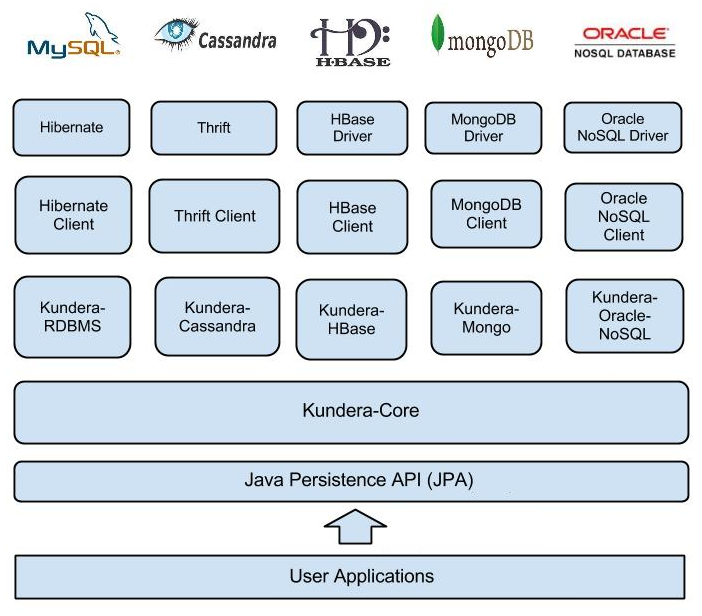
\includegraphics[scale=0.5]{images/kundera_architecture}
  \caption{Kundera architecture}
  \label{fig:kundera_architecture}
\end{figure}

\noindent The architecture of Kundera is shown in Figure \ref{fig:kundera_architecture}. The figure highlights the fact that the user application interacts with Kundera simply by exploiting the standard JPA interface implemented in the Kundera-Core.

\noindent Kundera-Core, each time an operation need to be executed on the underlying database, delegates the operation to the appropriate \texttt{Client} (creating it through a \texttt{Client Factory} if it does not exists yet). Clients are then responsible of actually executing the operation on the underlying database.

\subsection{Kundera's Client Extension Framework}
Kundera tries to offer a common way to interact with NoSQL databases through a well defined interface furthermore, since it is as on open source project, it makes other developers able to extend it, adding support for other databases.
The \textit{Client Extension Framework}, described in the Kundera documentation, provides a short description about how Kundera clients should work and gives a description of interfaces and classes that should be developed in order to make the client work properly.

\newparagraph Basically to build a new Kundera client, these are the blocks to be developed:
\begin{itemize}
\item the \texttt{Client}, which is the gateway to CRUD operations on database, except for JPQL queries and named queries;
\item the \texttt{Client Factory}, which is used by Kundera to instantiate the new Client;
\item the \texttt{Query implementor}, which is used by Kundera to run JPA queries by invoking appropriate methods in Entity Readers;
\item the \texttt{Entity Reader}, which is used by Kundera to translate the queries into correct client method calls;
\item optionally the \texttt{Schema Manager}, to support automatic schema generation.
\end{itemize}

\subsection{Approaching the extension}
While trying to extend Kundera we faced several problems that were not covered by the documentation.

\newparagraph TODO

\newparagraph It all seems well structured but the problem is that the documentation is actually outdated. 
\noindent Two were the main problem in understating what to do and how:
\begin{itemize}
\item when actually defined the classes and implemented the interfaces, it turns out that there are actually little differences both on interfaces and the required methods 
\item the documentation skip completely to describe what kind of information are carried by the argument of the methods that needs to be implemented
\end{itemize} 

\noindent Due to those problems, the solution was to write on the Kundera Google group page to ask the community for more updated information about Kundera extension.
Briefly an answer has come and I've started a conversation with one of the developers of Kundera who helped me giving the updated information for the Kundera's \textit{Client Extension Framework} and tell me to look forward to the other client implementation for some examples. 
Thanks to the updated information it turns out that the \texttt{Entity Reader} was unnecessary and all the translation from JPA queries to datastore specific queries and their executions should be done in the \texttt{Query Implementor}.  

\newparagraph At this point since no answer were given about the information carried by the methods arguments, the most valid solution was to approach the extension in a test driven way trying so to reverse engineer the arguments.

\noindent Looking at the tests code of the other clients, I've written a set of unit tests one for each feature I was planning to support (tests are analyzed in chapter \ref{chap:eval}).
By doing this and by looking at the other client implementation I was finally able to understand the structure of the method arguments, they carry information about the operation to be performed and about the entity on which the entity needs to be performed.
Entity information are structured in a data structure filled by Kundera by parsing the annotation that the user define on the entity class, those meta-data includes for example the table name, the column names and the relationships in which the entity is involved.

\noindent With the client structure defined, the tests written, the knowledge of the responsibilities of each method and of the Kundera meta-model, was then possible to begin the actual extension developing.

\section{Developing client extensions}
\label{sec:develop}
The work carried out has also focused on the development of two Kundera extensions, the first one for Google Datastore and the second one for Azure Tables.

\noindent Kundera \textit{Client Extension Framework} provides a generic interface which methods are supposed to carry out a lot amount of code, an example of this is the persist operation that is handled by the \texttt{onPersist} method, besides actually perform the persist operation, have to create an object that can be persisted by reading all the entity meta-data given as arguments and looking as example to relational fields.
\noindent The adopted solution is a template pattern in which each method maintains the main algorithm structure and delegates every operation to a specific hook method.
An example of this approach for the Datastore case, is reported in pseudo code in the snippet \ref{code:approach}.

\begin{lstlisting}[language=Java, caption=Template for the persist operation, label=code:approach]
@Override
protected void onPersist(...) {
    Entity gaeEntity = DatastoreUtils.createEntity(entityMetadata, id);
    handleAttributes(gaeEntity, entityAttributes);
    handleRelations(gaeEntity, relationHolders);
    handleDiscriminatorColumn(gaeEntity, entityMetadata);
    performPersist(gaeEntity);
}
\end{lstlisting}

\noindent For the Azure Tables extension, since it has been developed as the last one, the same structure has been kept and so it was only necessary to update the code of the hook methods.

\noindent The following sections presents these extensions separately, each feature developed is described in a dedicated section

\subsection{Google App Engine Datastore client}
\label{sec:kundera-datastore}
Google App Engine Datastore \cite{online:datastore} is the NoSQL solution build on top of Google BigTable a sparse, distributed, persistent multidimensional sorted map available in the App Engine platform. 

\subsubsection{JPA identifier}
The most basic unit that can be stored in Google Datastore is an \textit{Entity}, which is identified by a \textit{Key} and it is composed by \textit{Properties}.
Keys contain various information about the entity itself:
\begin{itemize}
\item the entity \textit{Kind}, which is used to group entities of the same type;
\item an entity identifier, used to distinguish entities of the same type;
\item an optional parent entity .
\end{itemize}
Inspired by the Google JPA implementation for Datastore \cite{online:googlejpa} the idea was to use the Java class representing the datastore \textit{Key} as identifier for the entity, but, unfortunately, this was not possible since Kundera support only a pre-defined defined set of Java data types.

\noindent Hence the adopted solution is to handle the key internally. Each time an operation on Datastore is required the key, relative to the entity, is built. The \textit{Kind} is directly mapped to the table name and the Key identifier is the user defined id specified in the \texttt{@Id} annotation.

\newparagraph TODO spiegare \texttt{@Id} 

\newparagraph IDs can be specified by the user or automatically generated, and they can be associated to three different datatypes
\begin{itemize}
\item \texttt{@Id} annotation on a \texttt{String} type field
\item \texttt{@Id} annotation on a \texttt{Long} type field
\item \texttt{@Id} annotation on a primitive \texttt{long} type field
\end{itemize}

\noindent Since Kundera supports the JPA feature for auto-generated IDs by using the annotation \texttt{@GeneratedValue}, this possibility has been exploited also for Datastore and so the user can annotate a \texttt{String} ID field so as that it will be auto-generated and its value will be a string representation of a random java \texttt{UUID}.

\noindent Auto-generated IDs are supported by Kundera only with \texttt{AUTO} or \texttt{TABLE} strategy, it was not possible to use the Datastore API to generate IDs since it is necessary to know the \textit{Kind} of the entity to be persisted but neither the \texttt{AUTO} strategy nor the \texttt{TABLE} one provides this information at generation time.

\subsubsection{Consistency}
In Datastore entities are organized in \textit{Entity Groups} based on their \textit{Ancestor Path}. The Ancestor Path is a hierarchy of entities whose keys have relation among themselves.

\noindent Consistency is managed through entity groups and so by defining the ancestor paths. Entities within the same entity group are managed in a strongly consist TODO. Entities which are not in an entity group are treated with eventual consistent policy.

\noindent Datastore allows to create ancestor paths by defining entities parental relationships between entities and is it a task left to the user. Datastore low-level API also leave this task to the user, for example in Objectify \cite{online:objectify}, a wrapper for these API, the developer makes use of a \texttt{@Parent} annotation to make the user able to specify the parent relationships and hence to be able to organize entities through the ancestor path.

\noindent Since JPA is a well defined standard, adding such kind of annotation will break the standard and the only alternative left is trying to automatically guess the ancestor path.

\noindent An approach to do so can be to look at JPA relationships since they are clearly a good place to found information for guessing if two entity kind can be hierarchically related, hence for each type of relation we may define some solutions that can be adopted:
\begin{itemize}
\item for \textbf{One to Many} and \textbf{One to One} relationships, since there is an owning side of the relationship, the owning entity can be used as parent for every related entity. 
\item \textbf{Many to One} relationships can be considered as \textbf{One to Many} relationships. 
\item as regards \textbf{Many to Many} relationships, since the each one is typically used by performing a join operation on a join table \dots TODO spiegare perchè non ha senso
\end{itemize}

\noindent Eventhough it could have been possible to infer such relationships we choose not to implement it inside the Kundera extension for two main reasons: 
\begin{enumerate}
\item entities are not require to have a single relationship
\item entities with a parent require the parent Key to be universally identified
\end{enumerate}
So for the first reason is impossible, unless asking to the user, to decide which relation use to hierarchically organize entities, furthermore for the second reason when declaring a entity parent to another is always necessary to know the Key of the parent (and thus its Kind and identified) beside the Key of the entity itself to be able to retrieve it from Datastore and for how Kundera is structured this information is not available during find operation in which Kundera provides only the table name, the identifier and the entity class.

\newparagraph For those reasons was not possible, without causing errors, to automatically guess ancestor paths through JPA relationships or make the user able manage them directly through a specific annotation.
Each Kind is persisted as a root Kind and so each entity is stored in a separated entity group identified by its Kind (the name of the JPA table associated to the entity).

\subsubsection{JPA relationships}
All the JPA supported relationships has been implemented in the client and  have been implemented like they would be in a relational database.
So for \textbf{One to One} and \textbf{One to Many} relationships on the owning side of the relationships a \textit{reference} to the non-owning side entity is saved.

\noindent For \textbf{Many to One} relationships there would be two solutions:
\begin{itemize}
\item persist a list of \textit{references} to the related entities;
\item do not persist anything within the entity and fill the relationship with a query.
\end{itemize}
The second solution has been adopted since more consistent with other Kundera client implementation and with the classic implementation of this relation type in relational systems.

\noindent For \textbf{Many to Many} relationships a join table is created based on user directives specified in the entity class annotations. The join table is filled each time a many to many related entity is persisted and a new \textit{row} is created inside the join table with the \textit{references} to the entities involved in the relationship.

\noindent The so far called \textit{reference} for Datastore is exploited by persisting within the entity the Key (Kind and identifier) of the related entity.

\subsubsection{Queries}
Queries in Kundera are supported in JPQL the JPA query language which is a  object oriented query language based on SQL \cite{book:projpa2}.
Kundera supports all of the clauses of JPQL but with some restrictions, clauses can be applied on:
\begin{itemize}
\item primary key attributes (\texttt{@Id}) and column attributes (\texttt{@Column}).
\item combination for primary key attribute and columns.
\end{itemize}

\noindent The JPQL query is parsed and validated by Kundera and to the \texttt{Query Implementor} are provided some meta-data extracted from the query which then needs to be read in order to build a database specific compatible query.

    
\newparagraph Datastore have on its own a very good support to queries so all the clauses are supported except for the \textit{LIKE} clause.

\noindent To be able to execute queries on properties, Datastore needs to construct indexes upon those properties. Those indexes consumes the App Engine application quotas both to be stored and maintained. The API provides the possibility to decide upon which property an index should be maintained by using a different method when the property is added to the entity; \texttt{setProperty(String name, Object value)} is used to set a property which will be automatically indexed,  \texttt{setUnindexedProperty(String name, Object value)} will be used otherwise.

\noindent Since a discriminator is needed to choose between the two methods, other wrapper around low-level API such Objectify \cite{online:objectify} provides to the user an \texttt{@Index} annotation to be place upon the field that needs to be indexed but, as previously explained, is not convenient to add other annotation to the JPA standard, this will break interoperability. For those reasons, and to be able to actually execute the queries, all properties are set as indexed.

\newparagraph In table \ref{table:queries} can be found a complete list of the supported JPQL clauses for both extensions.

\subsubsection{Embedded entities}
Embedded fields are supported by the JPA \cite{book:projpa2} annotating the field that needs to be embedded with the \texttt{@Embedded} annotation and annotating the corresponding class with the \texttt{@Embeddable} annotation.

\newparagraph Implementation of those kind of entities is straightforward for Datastore because it supports them natively as an \textit{Embedded Entity}.
\noindent The implementation so make use of this feature translating the embeddable entity in a Datastore embeddable entity and then persist it within the parent entity.

\subsubsection{Collection fields}
JPA standard supports collection or maps to be used as entities field through the annotation \texttt{@ElementCollection}.

\newparagraph Lists are natively supported by Datastore but are supported only if composed of primitives Java data types.
\noindent To be able to save whatever kind of collection or map independently by the data type that compose it, the collection or map itself is serialized to a \texttt{byte} array when persisted and de-serialized when read.
\noindent To simplify the developing, also Lists of primitive types, even if supported natively, are serialized.

\subsubsection{Enum fields}
Enum fields are supported by the JPA through the annotation \texttt{@Enumerated}  simply by persisting its string representation and instantiating the corresponding enum type back when the entity is read.

\subsubsection{Schema Manager}
Schema manager as required by Kundera has to exploit four operations:
\begin{itemize}
\item \textit{validate}, which validates the persisted schema based on entity definition
\item \textit{update}, which updates the persisted schema based on entity definition
\item \textit{create}, which create the schema and thus the tables based on entity definitions
\item \textit{create\textunderscore drop}, which drops (if exists) the schema and then re-creates it by re-creating the tables based on entity definitions.
\end{itemize}

\noindent The first two cases are quite useless for a Datastore since there's no fixed schema for entities, entities with same \textit{Kind} can have different properties without restriction.
Also the \textit{create} case is meaningless for Datastore since if a new entity of an unknown \textit{Kind} is persisted it's created without the need of explicitly define it first as a new \textit{Kind}.

\noindent The last case \textit{create\textunderscore drop} will just drop the current schema, deleting all the persisted kinds and so all the related entities, without re-creating the schema since it constructs by itself.

\subsubsection{Datastore specific properties}
Kundera offers the possibility to define some datastore specific properties in an external xml file that need to follow a simple structure. This file is referenced inside the \texttt{persistence.xml} and is optional.

\newparagraph This possibility is exploited by the Datastore extension and make the user able to configure the following properties:
\begin{itemize}
\item \texttt{datastore.policy.read}, to set the read policy
\item \texttt{datastore.deadline}, to define the RPCs calls deadline
\item \texttt{datastore.policy.transaction}, to specify if Datastore have to issue implicit transactions
\end{itemize}
Those properties are read in the \texttt{Client Factory} and used to initialize the datastore connection with the required parameters.

\newparagraph For a complete reference for Google Datastore extension configuration see the appendix \ref{appendix:datastore-config}.

\subsection{Azure Table client}
\label{sec:kundera-table}
Azure Table \cite{online:azuretable} is the NoSQL solution developed by Microsoft, is a key-value storage and it's available inside Azure environment.

\subsubsection{JPA identifier}
In Azure Table an entity to be persisted must either implement a special interface \texttt{TableServiceEntity} or be translated into a \texttt{DynamicEntity} which is basically a property container.
An entity is then uniquely identified inside a table by a \textit{partition-key} and a \textit{row-key}.
\noindent Partition keys are used to handle consistency, strong consistency is guaranteed while entities are stored within the same partition key otherwise consistency will be eventual.

\noindent Since both partition-key and row-key are supported only in field of type \texttt{String} and since the JPA annotation \texttt{@Id} can be declared only on one field per class, partition-key and row-key are concatenated in a single \texttt{String} and handled internally by the extension through the class \texttt{AzureTableKey} built \textit{ad hoc} since for Azure Table there's no a class similar to \texttt{Key} of Datastore that encapsulate both the partition-key and the row-key.
\noindent This way the user have complete control over partition-key and row-key and thus on the consistency mechanism.

\newparagraph For the user three different approaches to handle those identifiers are available:
\begin{enumerate}
\item define manually both row-key and partition-key
\item define manually only the row-key 
\item let the extension to completely handle the identifier annotating the ID field also with \texttt{@GeneratedValue(strategy = GenerationType.AUTO)}
\end{enumerate}

\noindent For the first case, to help the user in defining both the partition key and the row key independently by the way the extension handle them, a static method \texttt{AzureTableKey.asString(String partitionKey, String rowKey)} is provided; its usage is not required but in case the ID is manually specified, it must follow the convention used by the extension which is \texttt{partitionKey\textunderscore rowKey}.

\noindent The second case is exploited setting the ID to a string value, this value is interpreted by the extension as the row key while the partition key is set to a default value that can be modified in the datastore specific property file described later on. Also for this case, to have a more fluent API, an utility method is provided: \texttt{AzureTableKey.asString(String rowKey)} 

\noindent The third and last method will generate a java random \texttt{UUID} for the row key and set the partition key to the default value.

\subsubsection{JPA relationships}
Also for Azure Table relationships are implemented similarly to relational systems as described previously for Datastore (\ref{sec:kundera-datastore}).

\noindent The only difference is that when is needed to keep a \textit{reference} to another entity, is persisted within the entity the partition key and the row key of the related entity.
Even if the pair (partition-key, row-key) is not sufficient to identify an entity universally, it is sufficient in Kundera since the information of the table is always available to the client just by looking at the meta-data of the relationship. 

\subsubsection{Queries}
Supporting queries for Azure Tables was straightforward, the procedure was the same described in \ref{sec:kundera-datastore} but due to the different operator supported by Tables, beside the \textit{LIKE} clause also the \textit{IN} and \textit{ORDER BY} clauses are not supported.

\noindent In table \ref{table:queries} can be found a complete list of the supported JPQL clauses for both extensions.

\subsubsection{Embedded entities}
Embedded fields (described in \ref{sec:kundera-datastore}) are not supported natively by Azure Table so the solution adopted is to serialize the field annotated with \texttt{@Embedded} to be able to persist it to the storage like a \texttt{byte} array and de-serializing it when the entity is read.

\subsubsection{Collection fields}
As described for Datastore (\ref{sec:kundera-datastore}) JPA supports collections but are not supported in Azure Tables even if composed of supported data types.

\noindent To support even complex collection or maps the simplest solution is to serialize the entire collection or map to a \texttt{byte} array when persisting the entity and de-serialize it when reading the entity from the storage.

\subsubsection{Enum fields}
Enum fields are supported by the JPA through the annotation \texttt{@Enumerated}  simply by persisting its string representation and instantiating the corresponding enum type back when the entity is read.

\subsubsection{Schema Manager}
Schema manager (as described in \ref{sec:kundera-datastore}) have been also implemented for Azure Table and like Google Datastore, the first two cases are quite useless since there's no fixed schema and entities within the same Table can have different properties without restriction.

\noindent Azure Table need that the Table in which entities are stored exists before trying to create entities so the \textit{create} case simply iterate over all table names and creates it in the database. 

\noindent For the \textit{create\textunderscore drop} case, all tables should be dropped (and so all the contained entities) and re-created. The problem here is that tables deletion is performed asynchronously and so exists an unpredictable amount of time in which the table cannot be re-created since it still exists even if not listed.
\noindent To overcome to this problem two solution can be adopted:
\begin{itemize}
\item catch the \texttt{StorageException} thrown when the table is created while still exists, put the process to sleep for an amount of time and then try again until success
\item do not delete the table itself but delete all its entities in bulk
\end{itemize}

\noindent The first method is clearly dangerous since no deadline is given or guaranteed for the table delete operation, the second solution is actually not so convenient because, even if deletion is performed as a batch operation, both the partition key and row key must be specified and thus one or more queries must be performed over the table to retrieve at least partition key and row key for each entity in the table, this will require an high number of API call and thus an high cost of usage.

\noindent So for the \textit{create\textunderscore drop} case is performed a drop of all the Tables and then are re-created even if this can cause the previously mentioned conflict, this option is left as is for testing purposes since in the storage emulator the problem is not showing because the Table storage is emulated over a SQL server instance.

\subsubsection{Datastore specific properties}
As described for Datastore (\ref{sec:kundera-datastore}), Kundera provides a datastore specific properties file that let the user set some specific configuration.

\noindent This possibility is supported also for Azure Tables with the following available properties:
\begin{itemize}
\item \texttt{table.emulator} and \texttt{table.emulator.proxy}, to make the user able to test against the local storage emulator on Windows
\item \texttt{table.protocol}, to make the user able to decide between \textit{HTTP} or \textit{HTTP} for storage API RPCs
\item \texttt{table.partition.default}, to let the user specify the value for the default partition key 
\end{itemize} 

\newparagraph For a complete reference for Azure Table extension configuration see the appendix \ref{appendix:table-config}.

\section{Summary}
In this chapter has been introduced in details how Kundera extension should been developed, the problem encountered during the development, how they've been addressed and the detail of the implementation of the two extensions including the feature that are currently supported.

\begin{table}[ht]
\begin{center}
\renewcommand{\arraystretch}{1.4}
\begin{tabular}{lcc}
\hline
\textbf{JPA-QL Clause} & \textbf{Datastore support} & \textbf{Table support}\\ 
\hline\hline
\textit{Projections}   & \cmark 	& \cmark 	\\ \hline
\textit{SELECT}        & \cmark 	& \cmark 	\\ \hline
\textit{UPDATE}        & \cmark 	& \cmark 	\\ \hline
\textit{DELETE}        & \cmark 	& \cmark 	\\ \hline
\textit{ORDER BY}      & \cmark 	& \xmark 	\\ \hline
\textit{AND}           & \cmark 	& \cmark 	\\ \hline
\textit{OR}            & \cmark 	& \cmark 	\\ \hline
\textit{BETWEEN}       & \cmark 	& \cmark 	\\ \hline
\textit{LIKE}          & \xmark 	& \xmark  	\\ \hline
\textit{IN}            & \cmark 	& \xmark  	\\ \hline
\textit{=}             & \cmark 	& \cmark 	\\ \hline
\textit{\textgreater}  & \cmark	& \cmark 	\\ \hline
\textit{\textless}     & \cmark 	& \cmark 	\\ \hline
\textit{\textgreater=} & \cmark 	& \cmark 	\\ \hline
\textit{\textless=}    & \cmark 	& \cmark 	\\ \hline
\end{tabular}
\end{center}
\caption{JPQL clauses support for the developed extension}
\label{table:queries}
\end{table}

